\paragraph*{}
  Nos équations décrivent notre fluide dans le domaine que nous avons défini mais ce n'est pas suffisant, il reste encore
  à définir comment notre fluide ce comporte aux frontières de notre domaine et comment il interagit avec notre domaine.
  
  En mécanique des fluides numérique il y as un jeu de condition aux bornes qui suffisent à décrire la majorité des   
  situations nous allons présenter ici celles que nous utiliserons dans nos simulations:
  
  \subsection{\bf Conditions périodiques :}
    Acclamé par la critique, les conditions périodiques aux bornes possèdent le bon goût d'être simples à implémenter et
    de ne présenter quasiment pas d'effet secondaire\footnote{Si ce n'est se placer dans un plan infini\dots}.
    
    \begin{figure}[hbtp]
      \centering
      \includegraphics[width=\linewidth]{periodic.pdf}
      \caption{Exemple de condition périodique matérialisée par les droites noires.}
      \label{fig:per}
    \end{figure}
  
    Dans ce cas il suffit de définir que les $f_i$ franchissant la frontière <<s'échangent>> avec leurs équivalents de
    la frontière rattaché, dans le cas de la figure \ref{fig:per} et avec les indices de la figure \ref{fig:ei} on peux     
    réécrire cela de manière plus formelle :
    
    $$
      \forall (\delta_x + \sign{e_{i,x}}) \in \Omega
    $$
    \begin{equation}     
      \begin{array}{rrcr}
        i \in [7,3,6] & f_i(\delta_x, 0) & \rightarrow & f_i(\delta_x + \sign{e_{i,x}}, 232),\\
        i \in [8,5,9] & f_i(\delta_x, 232) & \rightarrow & f_i(\delta_x + \sign{e_{i,x}}, 0),
      \end{array}
    \end{equation}
     avec $\Omega$ l'ensemble de la frontière considérée et $\sign{}$ la fonction qui renvoie le signe.



    \begin{figure}[hbtp]
      \centering
      \includegraphics[width=\linewidth]{iolet.pdf}
      \caption{Exemple de conditions d'entrée/sorties matérialisée par deux droites respectivement à gauche et à droite 
      du graphique.}
      \label{fig:iolet}    
    \end{figure}

  \subsection{\bf Entrée à vitesse imposée :}
    Quand il s'agit des entrées et de sorties il existe une référence dans le domaine et c'est l'article de
    Qisu Zou et Xiaoyi He\footnote{souvent abrégée en Zou \& He} \cite{Zou_1997}.
    Dans le cas de notre implémentation il nous à fallu les redémontrer dans le cadre des équations dimensionnées.
    
    L'idée est la suivante :
    Au niveau de l'entrée\footnote{Inlet en anglais (et dans la littérature en général).} dans le cas d'une entrée comme
    présentée dans la figure \ref{fig:iolet} après la diffusion $f_3, f_7, f_4, f_8, f_5$ son connus.
    On vas donc utiliser on les équations \ref{eq:rho} et \ref{eq:u} pour déterminer les inconnues $f_6, f_2, f_9$ et 
    $\rho$, si l'on écris explicitement les sommes des équations \ref{eq:rho} et \ref{eq:u} pour notre simulation $D2Q9$ 
    on obtiens :
    $$
      \rho = f_1 + f_2 + f_3 + f_4 + f_5 + f_6 + f_7 + f_8 + f_9,
    $$
    $$
      \rho u_x = c(f_2 - f_4 + f_6 - f_7 - f_8 + f_9),
    $$
    $$
      \rho u_y = c(f_3 - f_5 + f_6 + f_7 - f_8 - f_9).
    $$
     
    On peux réécrire ces équations pour faire apparaitre les $f_i$ inconnue d'un coté et les autres termes de l'autre :
    \begin{equation} \label{eq:zhrho}
      f_6 + f_2 + f_9 = \rho - (f_1 + f_3 + f_4 + f_5 + f_7 + f_8),
    \end{equation}      
    \begin{equation} \label{eq:zhux}
      f_6 + f_2 + f_9 = \frac{\rho u_x}{c} + ( f_4 + f_7 + f_8),
    \end{equation}
    \begin{equation} \label{eq:zhuy}
      f_6 - f_9 = \frac{\rho u_y}{c} - (f_3 - f_5 + f_7 - f_8).
    \end{equation}
    
    En soustrayant les equations \ref{eq:zhrho} et \ref{eq:zhux} et en réarrangeant les termes on obtiens :
    \begin{equation} \label{eq:rhozh}
      \rho = \frac{c}{c - u_x}(f_1 + f_3 + f_5 + 2( f_4 + f_7 + f_8)),
    \end{equation}
    étant donnée que l'on impose la vitesse $\u$ sur l'inlet l'équation \ref{eq:rhozh} nous donne la valeur de 
    l'inconnue $\rho$. Pour poursuivre le raisonnement il faut faire l'hypothèse\footnote{C'est là ou ce trouve le 
    <<tour de force>> de l'article \cite{Zou_1997}} que $f_2 - \feq_2 = f_4 - \feq_4$.
    Si l'on développe avec l'équation \ref{eq:feq} et \ref{eq:cs} cette hypothèse et que l'on simplifie on obtiens:    
    \begin{equation} \label{eq:f2zh}
      f_2 = f_4 + \frac{2\rho u_x}{3c}.
    \end{equation}
    Si l'on remplace \ref{eq:f2zh} dans \ref{eq:zhux} on obtiens :
    \begin{equation} \label{eq:f69zh}
      f_6 + f_9 =  \frac{\rho u_x}{3c} + f_7 + f_8,
    \end{equation}
    en sommant l'équation \ref{eq:f69zh} avec \ref{eq:zhuy} et en simplifiant on obtiens :
    \begin{equation} \label{eq:f6zh}
      f_6 =  f_8 + \frac{\rho}{2c}\left(\frac{u_x}{3} + u_y\right) + \frac{1}{2}(f_5 - f_3),
    \end{equation}
    la même chose en soustrayant l'équation \ref{eq:f69zh} avec \ref{eq:zhuy} et en simplifiant on obtiens :
    \begin{equation} \label{eq:f6zh}
      f_9 =  f_7 + \frac{\rho}{2c}\left(\frac{u_x}{3} - u_y\right) + \frac{1}{2}(f_3 - f_5),
    \end{equation}
    dans le cas d'un écoulement incompressible on peut prendre $\rho = 1$ ce qui permet encore de simplifier nos 
    équations.  
    Nous avons donc notre jeux d'équations suivant pour notre entrée :
    \begin{equation} \label{eq:vinlet}  
      \begin{array}{rcl}
        f_2 &=& f_4 + 2\dfrac{u_x}{3c},\\
        f_6 &=&  f_8 + \dfrac{1}{2}\left(\dfrac{u_x}{3c} + \dfrac{u_y}{c} + f_5 - f_3\right),\\
        f_9 &=&  f_7 + \dfrac{1}{2}\left(\dfrac{u_x}{3c} - \dfrac{u_y}{c} + f_3 - f_5\right).
      \end{array}
    \end{equation}
    
    \subsection{\bf Sortie à pression imposée :}
      Pour la sortie on suppose que $u_y = 0$ et que $\rho = \rho_\text{out}$, il nous reste à trouver les valeurs de 
      $u_x$ ainsi que de $f_7, f_4, f_8$ (dans le cas de la figure \ref{fig:iolet}).
      Avec le même raisonnement que précédemment et avec \ref{eq:rho} et \ref{eq:u} on obtiens :
      \begin{equation} \label{eq:zhorho}
        f_7 + f_4 + f_8 = \rho_\text{out} - (f_1 + f_2 + f_3 + f_5 + f_6 + f_9),
      \end{equation}      
      \begin{equation} \label{eq:zhoux}
        f_7 + f_4 + f_8 = \frac{\rho_\text{out} u_x}{c} + ( f_2 + f_6 + f_9),
      \end{equation}
      \begin{equation} \label{eq:zhouy}
        f_7 - f_8 = - f_3 + f_5 - f_6 + f_9.
      \end{equation}
      En soustrayant les equations \ref{eq:zhorho} et \ref{eq:zhoux} et en réarrangeant les termes on obtiens :
      \begin{equation} \label{eq:uxzh}
        u_x = c - \frac{c}{\rho_\text{out}}(f_1 + f_3 + f_5 + 2( f_6 + f_2 + f_9)),
      \end{equation}
      étant donnée que l'on impose la densité $\rho_\text{out}$ sur l'outlet l'équation \ref{eq:uxzh} nous donne la 
      valeur de l'inconnue $u_x$. 
      En réutilisant la même hypothèse et la même méthode que précédemment on obtiens :
      \begin{equation} \label{eq:f4zh}
        f_4 = f_2 + \dfrac{2\rho_\text{out} u_x}{3c},
      \end{equation}
      \begin{equation} \label{eq:f7zh}
        f_7 = f_9 + \dfrac{1}{2}\left( \dfrac{\rho_\text{out} u_x}{3c} + f_5 - f_3 \right),
      \end{equation}
      \begin{equation} \label{eq:f8zh}
        f_8 = f_6 + \dfrac{1}{2}\left(\dfrac{\rho_\text{out} u_x}{3c} + f_3 - f_5 \right).
      \end{equation}
      La encore dans le cas d'un écoulement incompressible on peut prendre $\rho_\text{out} = 1$ ce qui permet de 
      simplifier nos équations.  
      Nous avons donc notre deuxième jeux d'équations suivant pour notre sortie:
      \begin{equation} \label{eq:poutlet}  
        \begin{array}{rcl}
          u_x &=& c(1 - [f_1 + f_3 + f_5 + 2( f_6 + f_2 + f_9)]),\\
          f_4 &=& f_2 + \dfrac{2 u_x}{3c},\\
          f_7 &=& f_9 + \dfrac{1}{2}\left( \dfrac{u_x}{3c} + f_5 - f_3 \right),\\
          f_8 &=& f_6 + \dfrac{1}{2}\left(\dfrac{u_x}{3c} + f_3 - f_5 \right).
        \end{array}
      \end{equation}

    \begin{figure}[hbtp]
      \centering
      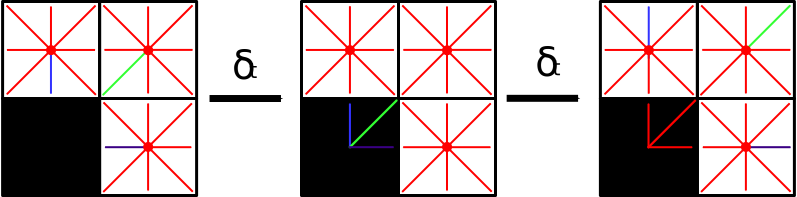
\includegraphics[width=\linewidth]{Fig/collide.pdf}
      \caption{Illustration du processus de collision avec un object (en noir).}
    \end{figure}     
    \subsection{\bf collision sans glissement :}

      Avec tout ce dons nous venons de discuter jusqu'ici il est évident que nous allons étudier un flux\footnote{Flow 
      Driven Analyses dans la littérature.}, mais pour l'instant nous n'avons pas encore discuté de l'interaction entre
      notre fluide et autre chose que lui-même.
      Les collisions sans glissement\footnote{Aussi appelées <<no slip boundaries>>.} peuvent s'interpréter de la 
      manière suivante : étant donnée une population de particules $f_i$ associée à une vitesse microscopique $\ei$ qui 
      rentre en collision avec un solide, elle va rebondir et repartir avec une vitesse $\ei$ opposée.
      Autrement dis pour simuler une collision il suffit d'échanger les populations $f_i$ de particules entre les 
      vitesses correspondante.
      Si l'on ce réfère à la figure \ref{fig:ei} nous avons les échanges suivants :
      \begin{equation}     
        \begin{array}{rcr}
          f_2 & \leftrightharpoons & f_4,\\
          f_3 & \leftrightharpoons & f_5,\\
          f_6 & \leftrightharpoons & f_8,\\
          f_7 & \leftrightharpoons & f_9,\\
        \end{array}
      \end{equation}
      $f_1$ correspondant aux particules au repos n'est pas échangé.
      

      
      